\chapter{RESULTS}\label{ch:results}

Sections~\ref{sec:verif}--\ref{sec:res-dev} cover development on the 96 training patients (patient-wise
cross-validation) and the verification of every implementation. Sections~\ref{sec:res-test}--\ref{sec:res-n8} cover
the single evaluation on the 29 held-out test patients after the design was frozen. Sections~\ref{sec:res-fpga}--%
\ref{sec:res-demo} cover the FPGA and the board.

\section{Verification of the Implementation}\label{sec:verif}

\begin{table}[H]
\centering\small
\caption{Verification of the integer front end and of the hardware}\label{tab:verif}
\begin{tabularx}{\textwidth}{|L|P{62mm}|}
\hline
\multicolumn{1}{|c|}{\textbf{Check}} & \multicolumn{1}{c|}{\textbf{Result}}\\
\hline
Integer features against the floating-point twin (10 training patients) & median correlation 0.9965; artefact flags
agree 99.7\,\%; LightGBM AUROC 0.736 vs 0.735\\
\hline
Verilog of the final DWN against the software (Icarus Verilog, 10 test recordings) & 431,960 windows, 0 mismatches
(features, bits, LUT outputs, scores, alarms)\\
\hline
Engine program (instruction-level simulator) against the C front end, 10 recordings & all 431,960 windows equal (38
features)\\
\hline
Engine RTL fed sample by sample (Verilator), EEG-only and all-sensor recording & 4,278 windows, 0 mismatches\\
\hline
Whole core from raw samples through AXI (Verilator) & 4,278 windows: features, score, decision and alarm equal\\
\hline
Whole core RTL regression with every fault injected & 863,920 checks and all 3,592 faults pass\\
\hline
\end{tabularx}
\end{table}

\section{Reproduction of the Published Baseline}\label{sec:res-chrononet}

\begin{figure}[H]
\centering
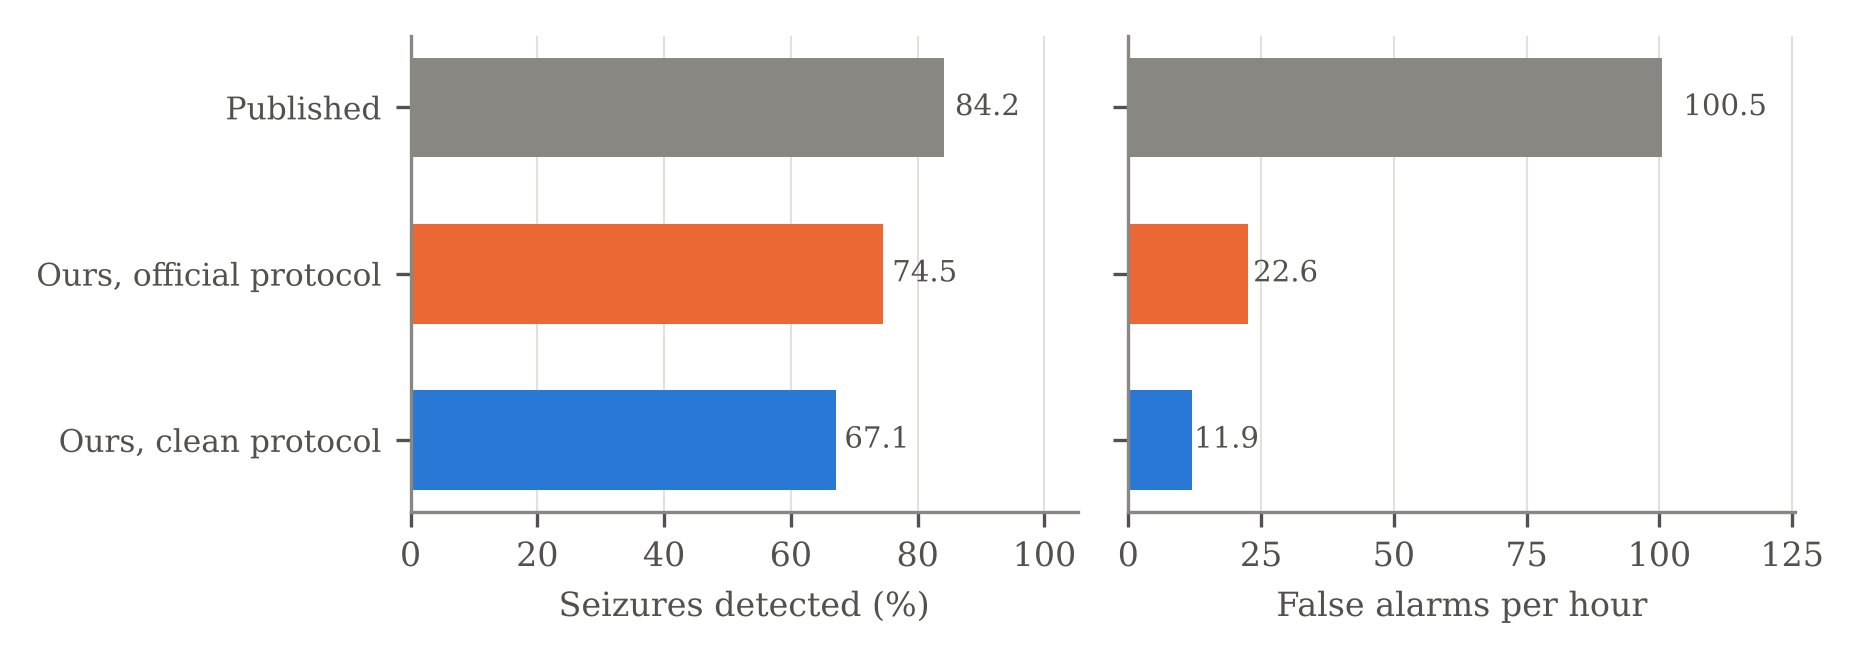
\includegraphics[width=0.9\textwidth]{figures/chrononet_repro.png}
\caption{ChronoNet on the 29 test patients: published and reproduced (the paper's metrics)}\label{fig:chrononet}
\end{figure}

\begin{itemize}
\item \textbf{Partly reproduced}: 74.5\,\% of seizures detected against 84.2\,\% published, with 22.6 instead of 100.5
  false alarms per hour (Figure~\ref{fig:chrononet}); the per-recording AUPR matches (0.109 vs 0.104).
\item \textbf{Test-set leak}: the released code picks its training epoch on the test patients. Our \textbf{clean} run
  (last epoch, no test information: 67.1\,\%, 11.9 false alarms per hour) is the reference for the final comparison.
\end{itemize}

\section{Model Development on the Training Patients}\label{sec:res-dev}

\begin{table}[H]
\centering\small
\caption{Five-fold cross-validation on the 96 training patients (best-F1 operating point)}\label{tab:families}
\setlength{\tabcolsep}{3pt}
\begin{tabularx}{\textwidth}{|P{36mm}|c|c|c|c|L|}
\hline
\multicolumn{1}{|c|}{\textbf{Model}} & \textbf{AUROC} & \textbf{Event-F1} & \textbf{FA/24\,h} & \textbf{Sens.\ $\le$1 FA/h} & \multicolumn{1}{c|}{\textbf{Estimated cost}}\\
\hline
LightGBM & 0.870 & 0.292 & 3.6 & 0.594 & $\approx$30.6k LUTs\\
\hline
CatBoost & 0.863 & 0.286 & 3.0 & 0.618 & $\approx$27.7k LUTs\\
\hline
XGBoost & 0.867 & 0.277 & 3.4 & 0.603 & $\approx$47.9k LUTs\\
\hline
TreeLUT & 0.857 & 0.266 & 4.2 & 0.619 & $\approx$6.4k LUTs\\
\hline
\textbf{DWN + distillation (final)} & 0.851 & \textbf{0.229} & \textbf{0.9} & 0.597 & \textbf{$\approx$870 LUTs}\\
\hline
DWN base & 0.840 & 0.211 & 2.4 & 0.581 & $\approx$960 LUTs\\
\hline
Random forest & 0.852 & 0.198 & 0.5 & 0.536 & $\approx$323k LUTs\\
\hline
Logic-gate network & 0.843 & 0.171 & 4.9 & 0.540 & $\approx$7.5k LUTs\\
\hline
INT8 MLP & 0.830 & 0.147 & 7.8 & 0.520 & 9,600 multiplications\\
\hline
Logistic regression & 0.806 & 0.105 & 8.8 & 0.409 & 117 multiplications\\
\hline
\end{tabularx}
\end{table}

The DWN is 7--8$\times$ smaller than the other LUT models and beats the INT8 MLP on every metric. Larger networks (up
to 2,000 LUTs), 16 thresholds, two layers and other temperatures gave no significant gain (Figure~\ref{fig:pareto});
4-input LUTs and 4 thresholds were clearly worse.

\begin{figure}[H]
\centering
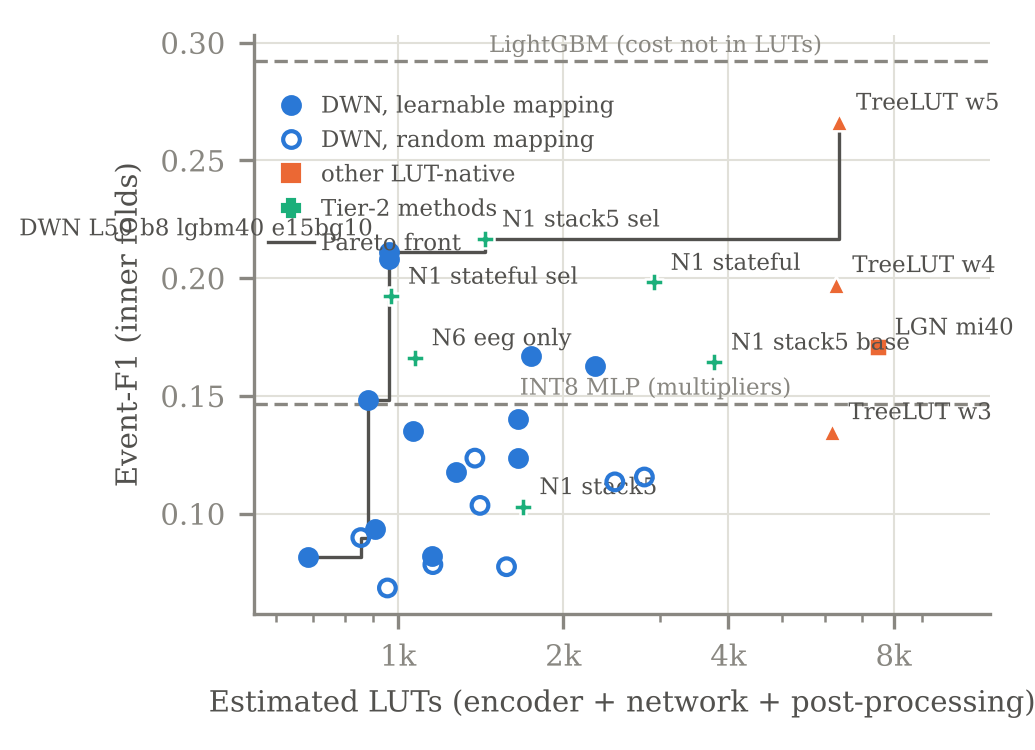
\includegraphics[width=0.66\textwidth]{figures/pareto_inner_cv.png}
\caption{Event-F1 against estimated LUTs for every LUT-native run (training folds), with the Pareto front}\label{fig:pareto}
\end{figure}

\begin{figure}[H]
\centering
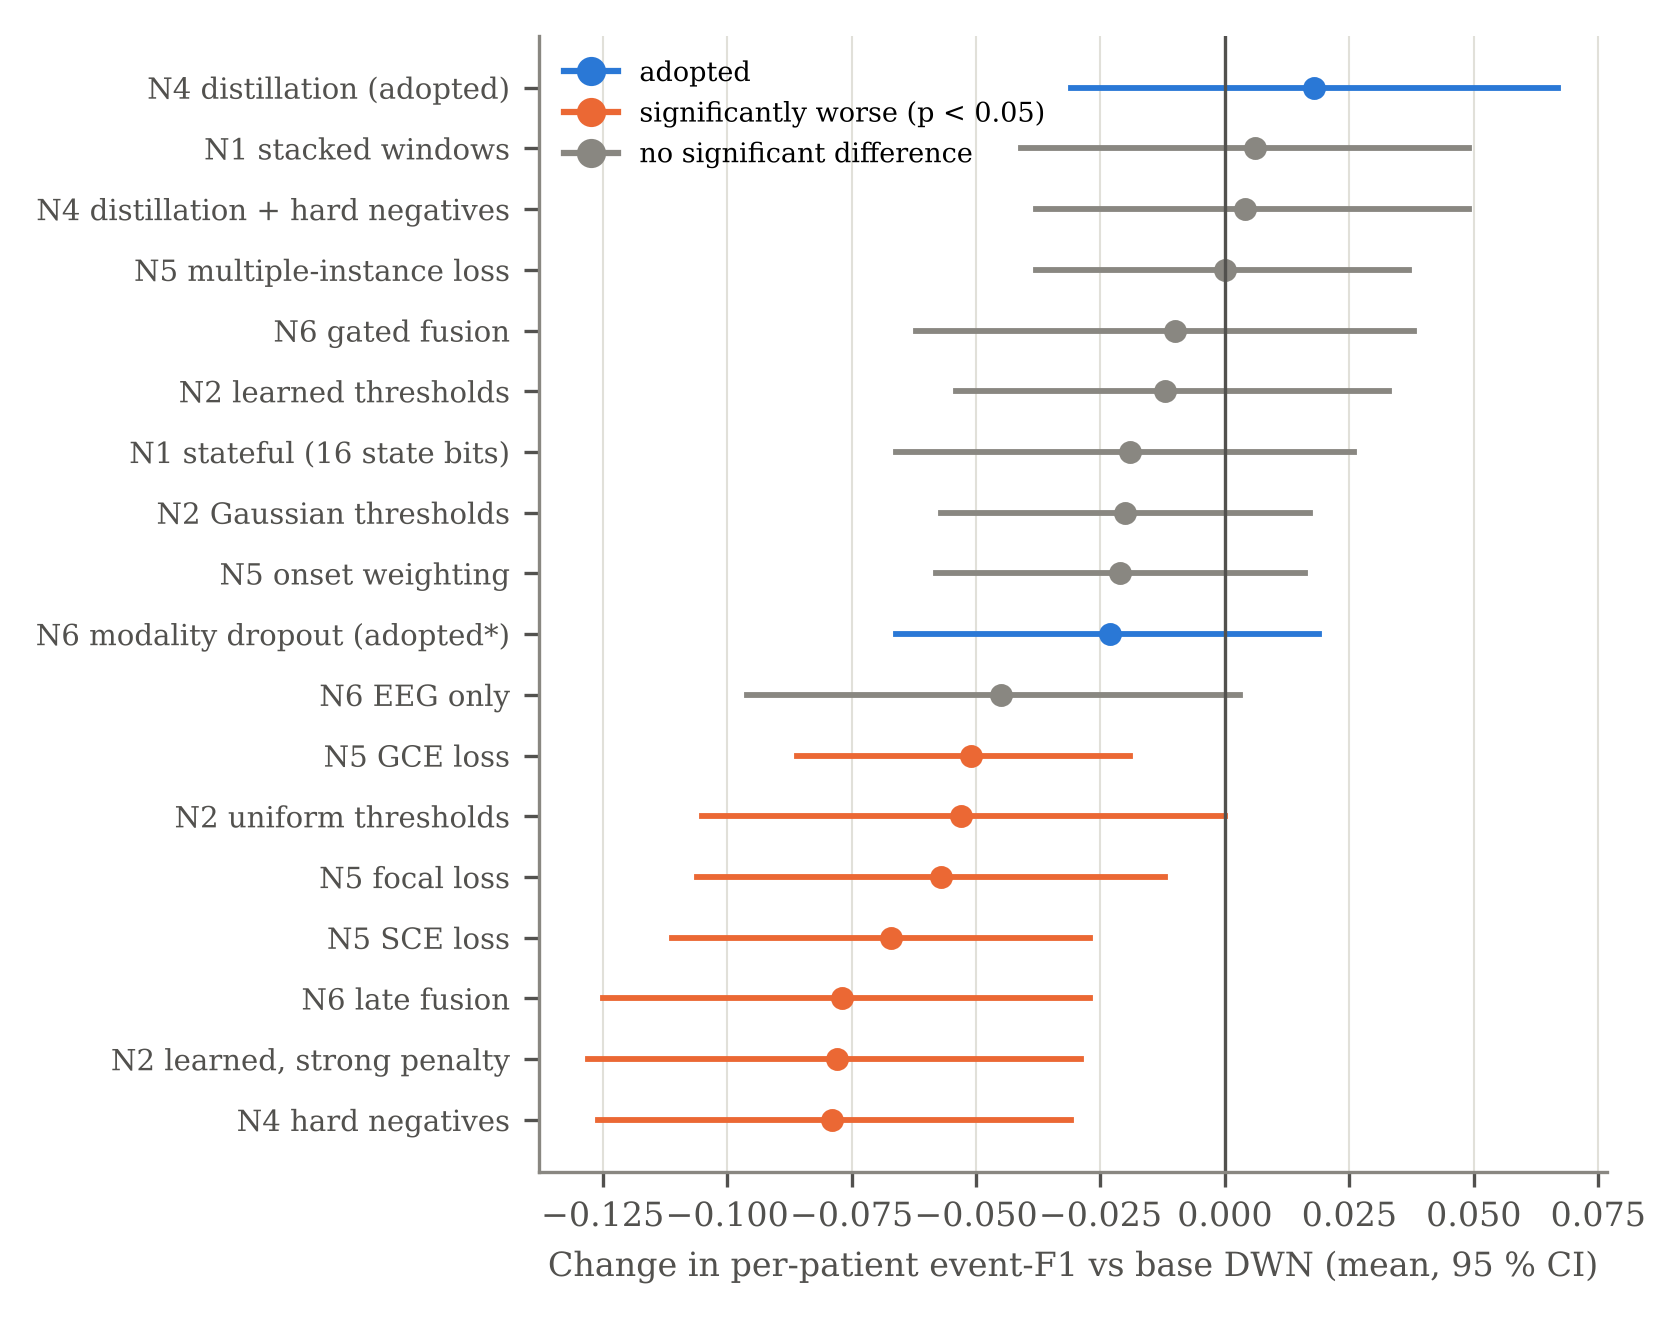
\includegraphics[width=0.85\textwidth]{figures/ablation.png}
\caption{Every extension against the base DWN: mean change in per-patient event-F1 with 95\,\% interval (modality
dropout was adopted for its robustness to missing sensors)}\label{fig:ablation}
\end{figure}

\begin{table}[H]
\centering\small
\caption{The changes that passed the significance test}\label{tab:adopted}
\begin{tabularx}{\textwidth}{|P{40mm}|L|P{34mm}|}
\hline
\multicolumn{1}{|c|}{\textbf{Change}} & \multicolumn{1}{c|}{\textbf{Evidence (training patients)}} & \multicolumn{1}{c|}{\textbf{How it was found}}\\
\hline
Feature selection by LightGBM importance & event-F1 0.148 $\to$ 0.208 ($p = 0.047$); false alarms 7.0 $\to$ 2.3/day & N7 showed the network ignored heart rate\\
\hline
Distillation from LightGBM (\textbf{final}) & false alarms 2.4 $\to$ 0.9/day ($p = 3\times10^{-7}$); event-F1 0.229 vs 0.211 & N4\\
\hline
Modality dropout (variant) & without ECG: event-F1 0.092 $\to$ 0.172 ($p = 0.005$) & N6\\
\hline
\end{tabularx}
\end{table}

\begin{figure}[H]
\centering
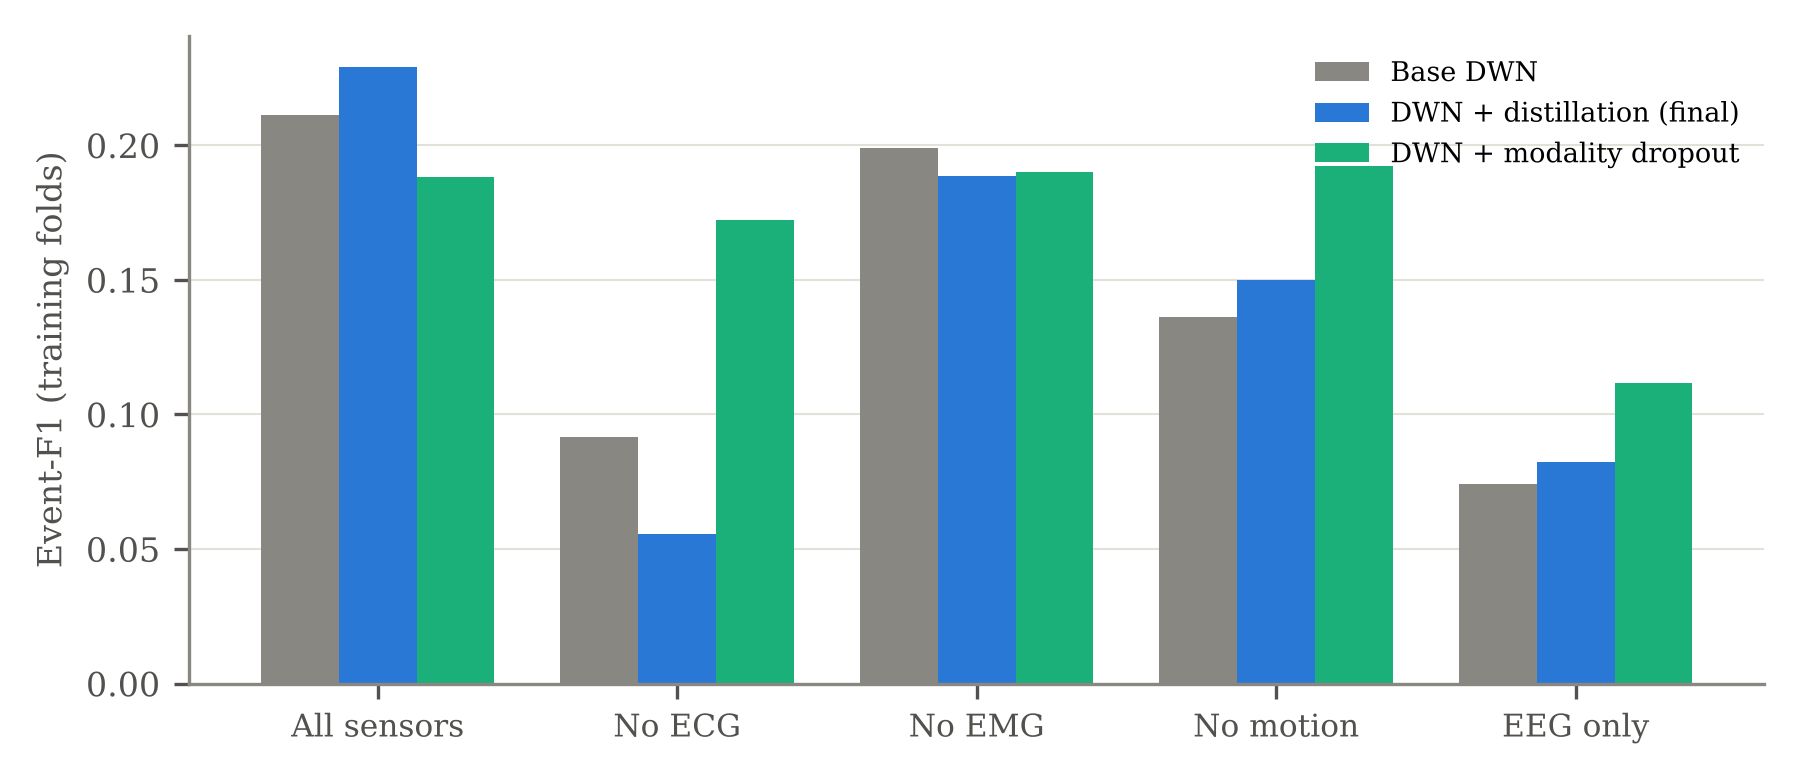
\includegraphics[width=0.85\textwidth]{figures/missing_sensors.png}
\caption{Event-F1 with sensors removed at test time (training folds): distillation is the most accurate with all
sensors; modality dropout keeps working without ECG or motion}\label{fig:missing}
\end{figure}

\begin{figure}[H]
\centering
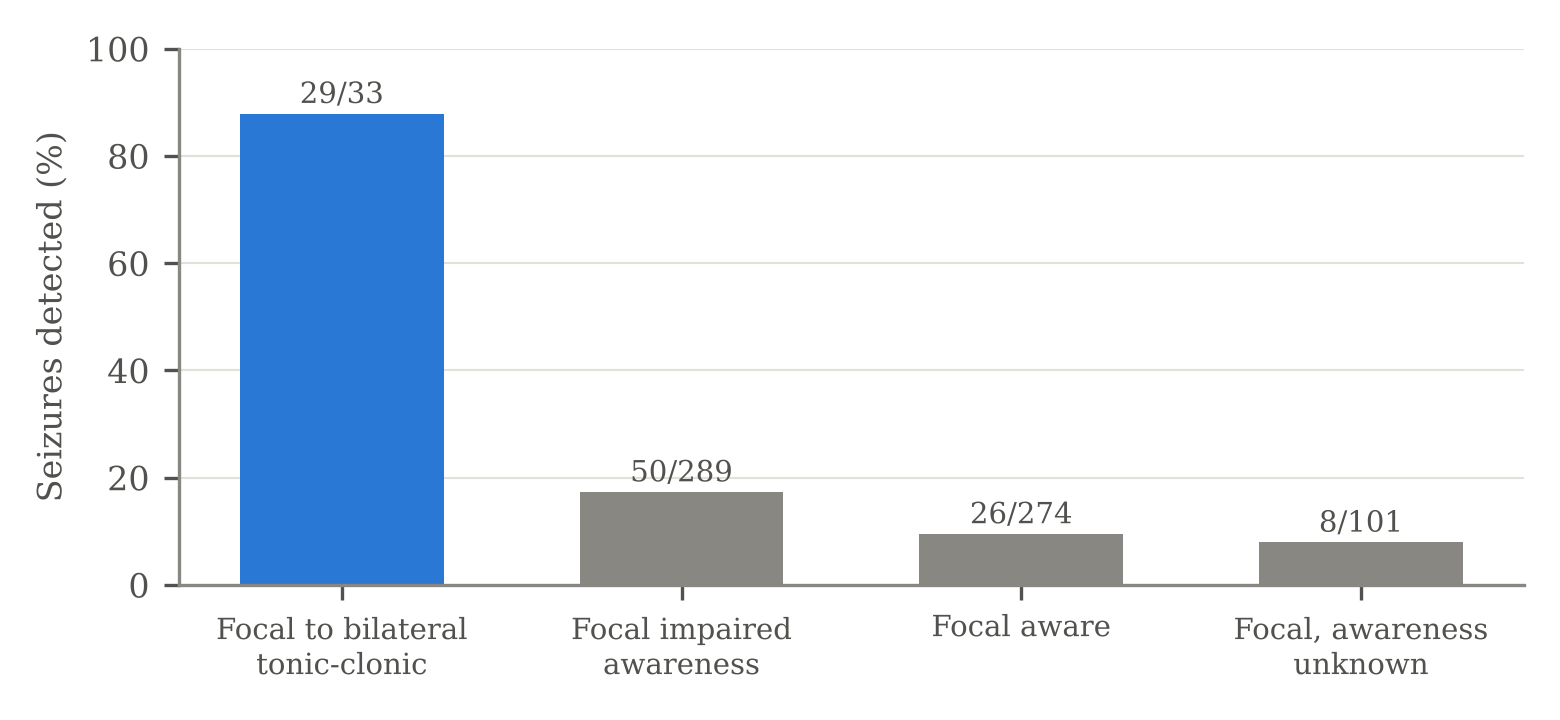
\includegraphics[width=0.62\textwidth]{figures/seizure_types.png}
\caption{Seizures detected by type (base DWN, training folds): tonic-clonic seizures are caught, focal seizures
rarely}\label{fig:types}
\end{figure}

\section{Final Evaluation on the Held-Out Test Patients}\label{sec:res-test}

\begin{figure}[H]
\centering
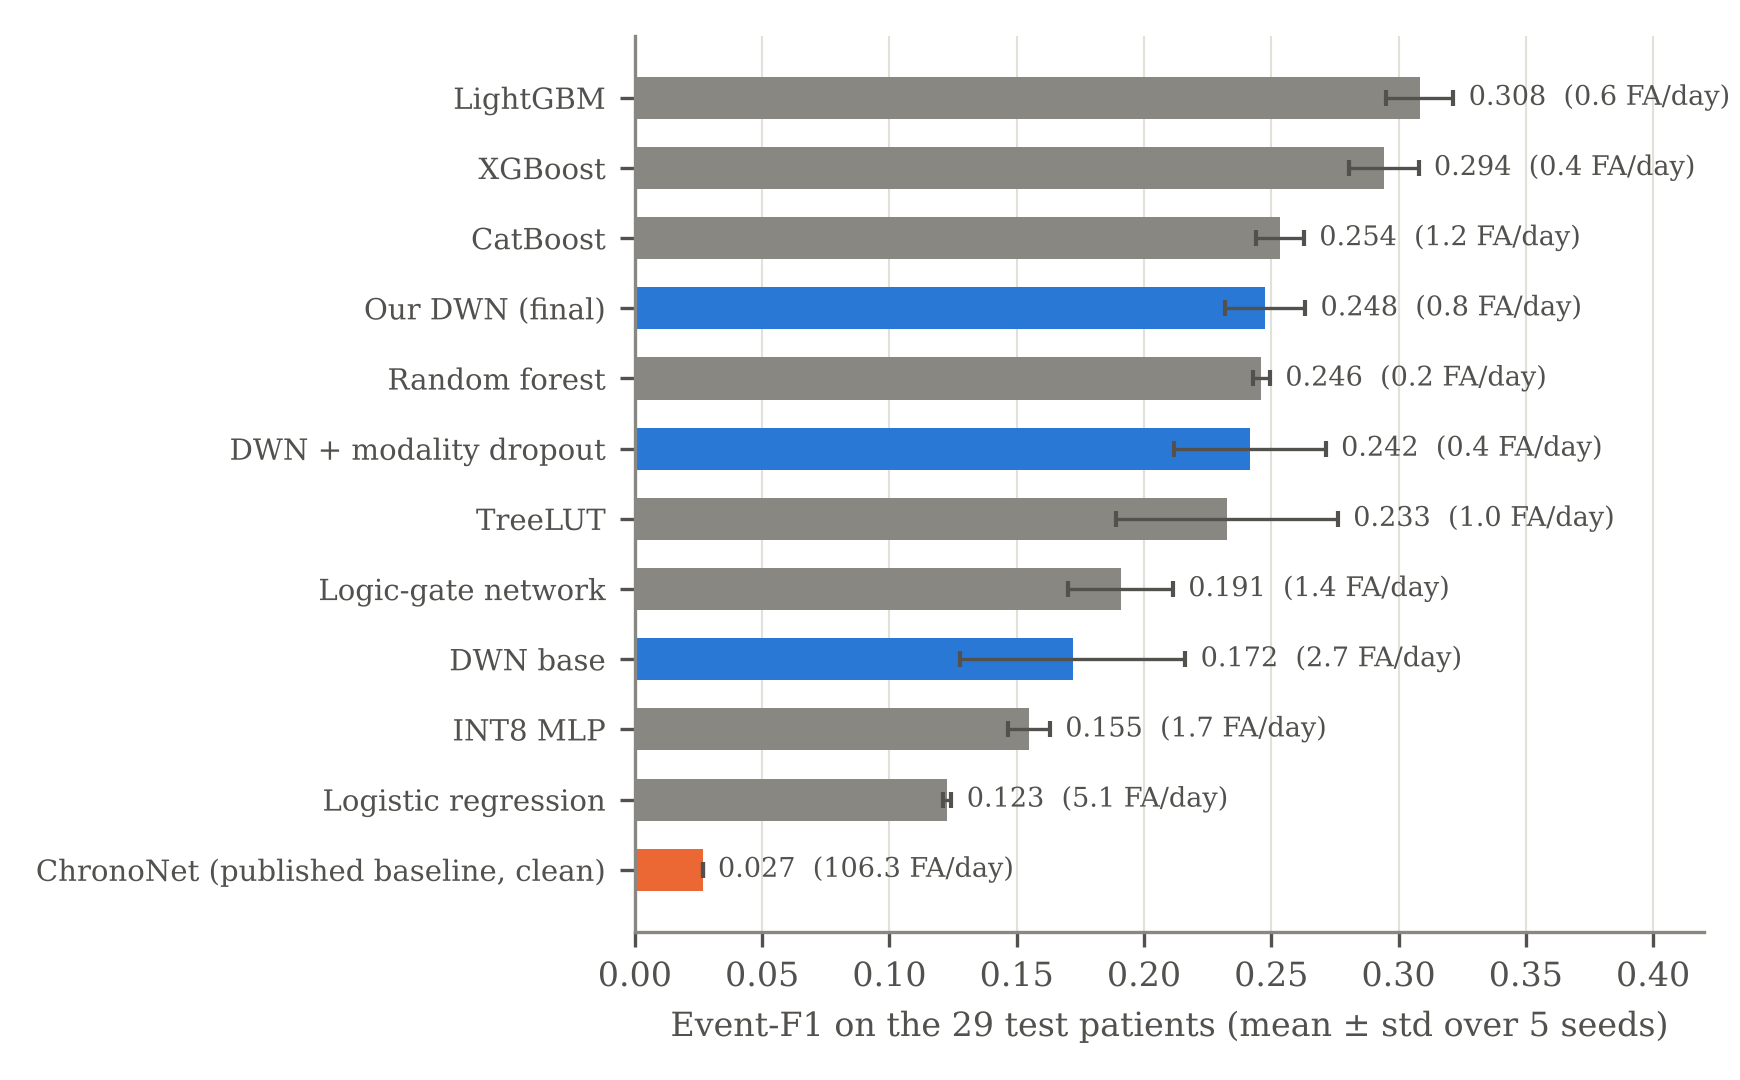
\includegraphics[width=0.85\textwidth]{figures/test_f1.png}
\caption{Event-F1 on the 29 test patients (mean $\pm$ std over 5 seeds) and false alarms per day}\label{fig:testf1}
\end{figure}

\begin{table}[H]
\centering\small
\caption{Final DWN against the main references on the 29 test patients ($p$: paired Wilcoxon on per-patient event-F1)}\label{tab:test}
\begin{tabularx}{\textwidth}{|P{40mm}|c|c|c|L|}
\hline
\multicolumn{1}{|c|}{\textbf{Model}} & \textbf{Event-F1} & \textbf{FA/24\,h} & \textbf{$p$ vs ChronoNet} & \multicolumn{1}{c|}{\textbf{Estimated cost}}\\
\hline
\textbf{DWN + distillation (final)} & \textbf{0.248 $\pm$ 0.016} & \textbf{0.8} & 0.027 & \textbf{$\approx$900 LUTs}\\
\hline
LightGBM & 0.308 $\pm$ 0.013 & 0.6 & 0.027 & $\approx$30.8k LUTs\\
\hline
CatBoost & 0.254 $\pm$ 0.009 & 1.2 & 0.031 & $\approx$27.7k LUTs\\
\hline
Random forest & 0.246 $\pm$ 0.003 & 0.2 & 0.27 & $\approx$347k LUTs\\
\hline
TreeLUT & 0.233 $\pm$ 0.044 & 1.0 & 0.016 & $\approx$6.3k LUTs\\
\hline
Logic-gate network & 0.191 $\pm$ 0.021 & 1.4 & 0.034 & $\approx$7.5k LUTs\\
\hline
INT8 MLP & 0.155 $\pm$ 0.008 & 1.7 & 0.017 & 9,600 multiplications\\
\hline
ChronoNet (clean) & 0.027 & 106 & -- & CNN + GRU\\
\hline
\end{tabularx}
\end{table}

The result held on unseen patients (0.248, above the cross-validation value of 0.229). The final DWN scores above
TreeLUT, the logic-gate network and the INT8 MLP, is level with random forest and CatBoost at 30--390$\times$ fewer
LUTs, and is significantly better than ChronoNet; LightGBM remains ahead ($p = 0.039$). All models are listed in
Appendix~\ref{app:results}.

\begin{figure}[H]
\centering
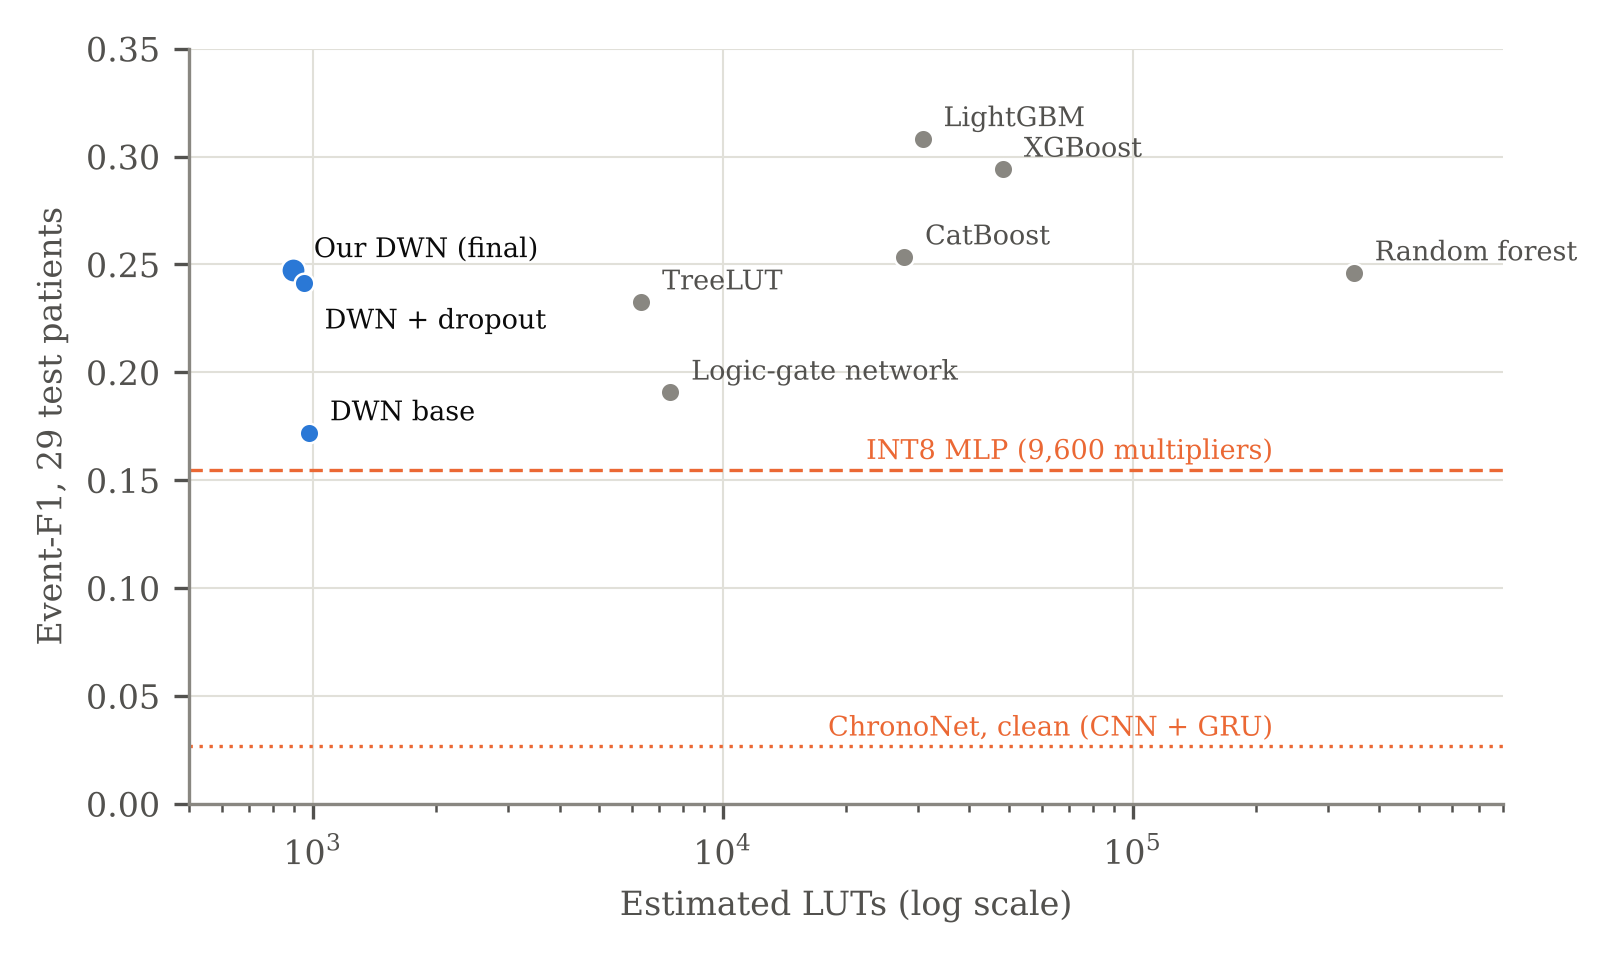
\includegraphics[width=0.78\textwidth]{figures/test_f1_vs_luts.png}
\caption{Accuracy against hardware cost on the test patients: the LUT networks reach tree-ensemble accuracy at a
fraction of the LUTs}\label{fig:testluts}
\end{figure}

\section{Comparison with the Base Paper}\label{sec:res-published}

\begin{figure}[H]
\centering
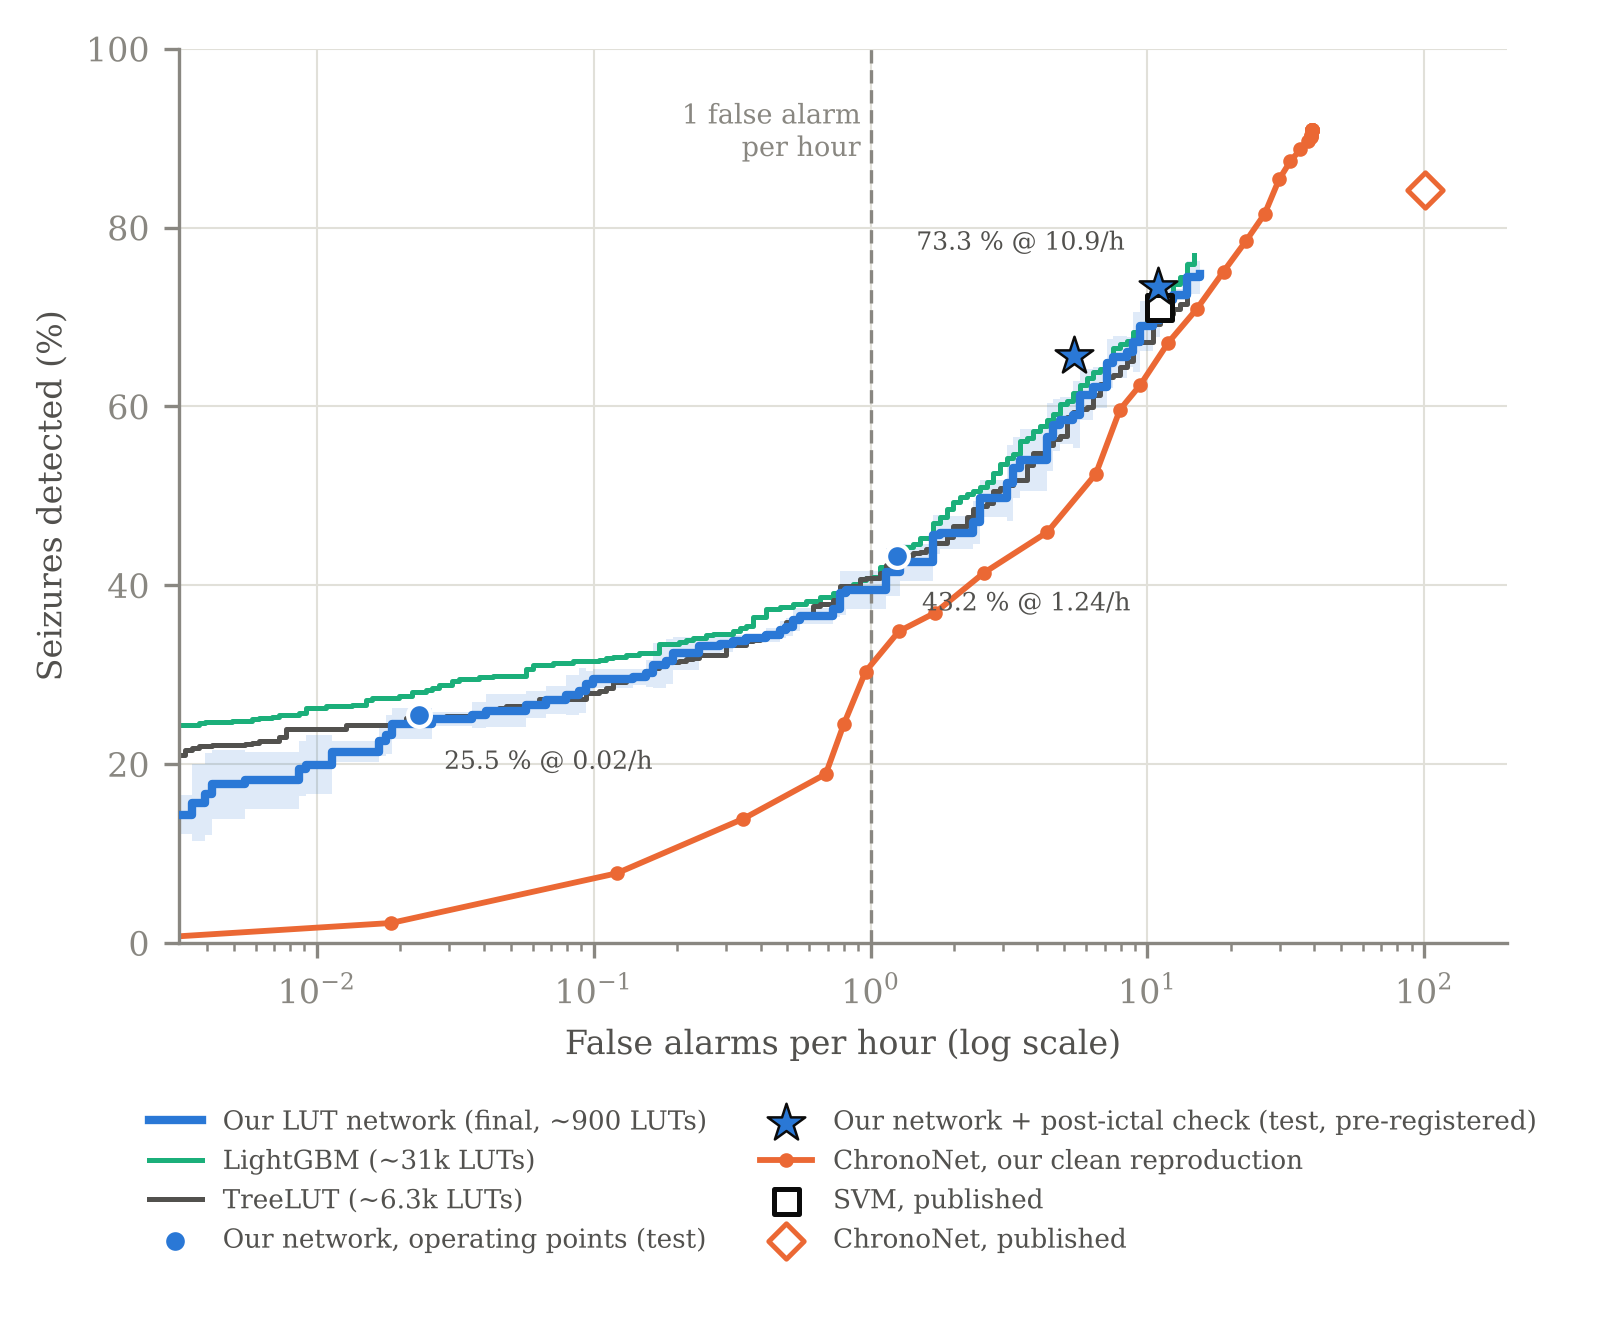
\includegraphics[width=0.82\textwidth]{figures/sens_fa_test.png}
\caption{Seizures detected against false alarms per hour on the 29 test patients (the base paper's metrics): threshold
sweeps of the frozen models, our operating points chosen on the training folds, the two-stage detector (stars) and the
published values (open markers)}\label{fig:sensfa}
\end{figure}

\begin{table}[H]
\centering\small
\caption{The base paper's baselines and our network on the same 29 test patients (the paper's metrics)}\label{tab:published}
\begin{tabularx}{\textwidth}{|L|c|c|c|}
\hline
\multicolumn{1}{|c|}{\textbf{Model}} & \textbf{Detected} & \textbf{FA/h} & \textbf{AUROC}\\
\hline
SVM, published \cite{bhagubai2025seizeit2} & 71.1\,\% & 11.0 & 0.700\\
\hline
ChronoNet, published \cite{bhagubai2025seizeit2} & 84.2\,\% & 100.5 & 0.792\\
\hline
ChronoNet, our clean reproduction & 67.1\,\% & 11.9 & 0.746\\
\hline
ChronoNet at $\approx$1.3 FA/h (threshold read from its own test curve) & 34.8\,\% & 1.26 & --\\
\hline
\textbf{Our DWN, $\le$1 FA/h operating point} & \textbf{43.2\,\%} & \textbf{1.24} & \textbf{0.883}\\
\hline
\textbf{Our DWN, best-F1 operating point} & \textbf{25.5\,\%} & \textbf{0.02} & \\
\hline
\textbf{Our DWN + post-ictal check (pre-registered, Section~\ref{sec:res-n8})} & \textbf{73.3\,\%} & \textbf{10.9} & \\
\hline
\textbf{Same, stricter verification} & \textbf{65.6\,\%} & \textbf{5.4} & \\
\hline
\end{tabularx}
\end{table}

The paper's baselines run at 11--100 false alarms per hour. At the same false-alarm rate our network detects more
seizures than ChronoNet (43.2\,\% against 34.8\,\% at about 1.25 per hour; 25.5\,\% against 2.2\,\% at about 0.02 per
hour), ranks windows better (AUROC 0.883 against 0.746) and needs no multipliers.

\section{Post-Ictal Verification}\label{sec:res-n8}

A two-stage detector (N8), requested after the final test, runs the final network at a sensitive threshold and
confirms each alarm 96\,s later with a second LUT network (50 LUTs) that compares the alarm with the minutes before and
after it. All settings were chosen on the training patients and committed before one evaluation on the test patients.

\begin{table}[H]
\centering\small
\caption{Two-stage detector: training patients (cross-validation) and test patients (5 seeds, paper's metrics)}\label{tab:n8}
\begin{tabular}{|l|c|c|c|c|}
\hline
\multicolumn{1}{|c|}{\textbf{Detector}} & \multicolumn{2}{c|}{\textbf{Training (CV)}} & \multicolumn{2}{c|}{\textbf{Test}}\\
\hline
 & Detected & FA/h & Detected & FA/h\\
\hline
Final network, lower threshold & 74.2\,\% & 8.5 & 66.4 $\pm$ 2.0\,\% & 7.6\\
\hline
\textbf{+ post-ictal check ($\le$10 FA/h)} & 81.9\,\% & 9.6 & \textbf{73.3 $\pm$ 1.4\,\%} & \textbf{10.9}\\
\hline
+ post-ictal check ($\le$5 FA/h) & 72.3\,\% & 4.8 & 65.6 $\pm$ 1.0\,\% & 5.4\\
\hline
SVM, published \cite{bhagubai2025seizeit2} & -- & -- & 71.1\,\% & 11.0\\
\hline
\end{tabular}
\end{table}

At the SVM's false-alarm rate (10.9 against 11.0 per hour) the LUT-native two-stage detector detects 2.2 points more
seizures, with all 5 seeds above 71.1\,\%. The costs are a 96\,s decision delay and many false alarms per day, as for
the paper's baselines, so the low-false-alarm result of Section~\ref{sec:res-test} remains the primary one.

\section{FPGA Implementation Results}\label{sec:res-fpga}

\begin{table}[H]
\centering\small
\caption{Cost of the LUT-native classifiers on the XCK26 (Vivado 2026.1 out of context, 2.5-ns constraint,
vectorless power at 400\,MHz; Yosys as a second flow)}\label{tab:hwcost}
\begin{tabular}{|l|r|r|r|r|r|r|}
\hline
\multicolumn{1}{|c|}{\textbf{Model}} & \textbf{LUTs} & \textbf{FFs} & \textbf{Fmax} & \textbf{Dyn. power} & \textbf{Yosys LUTs} & \textbf{Test F1}\\
\hline
\textbf{DWN + distillation (ours)} & \textbf{398} & 454 & \textbf{468\,MHz} & \textbf{17\,mW} & 405 & 0.248\\
\hline
TreeLUT (5-bit leaves) & 2,677 & 1,461 & 294\,MHz & 88\,mW & 2,721 & 0.233\\
\hline
Logic-gate network & 5,249 & 2,208 & 154\,MHz & 523\,mW & 5,758 & 0.191\\
\hline
\end{tabular}
\end{table}

\begin{table}[H]
\centering\small
\caption{Post-implementation utilisation of the whole detector and the KV260 design (Vivado 2026.1)}\label{tab:whole}
\begin{tabularx}{\textwidth}{|L|P{75mm}|}
\hline
\multicolumn{1}{|c|}{\textbf{Part}} & \multicolumn{1}{c|}{\textbf{Cost}}\\
\hline
Feature engine alone (out of context) & 804 LUTs, 101 FFs, 4.5 block RAMs, 0 DSP, 234\,MHz\\
\hline
Whole detector (feature engine + DWN) & \textbf{1,202 LUTs, no multiplier} (Yosys: 797 + 405, also 1,202)\\
\hline
Whole core in the design (with BIST, fault injection, debug, demo I/O) & 3,356 LUTs, 13.5 block RAMs\\
\hline
Full KV260 design & 3,796 LUTs (3.2\,\% of the device), 0 DSP; timing met at 100\,MHz (slack 3.5\,ns)\\
\hline
\end{tabularx}
\end{table}

The DWN needs 6.7 times fewer LUTs than TreeLUT and 13.2 times fewer than the logic-gate network, and it is also the
fastest. Its thermometer comparators, not the network itself, take most of its cost.

\section{Self-Test Results}\label{sec:res-bist}

\begin{table}[H]
\centering\small
\caption{Single faults on the training data and the decision-relevant faults detected (\%) by three self-test vector
sets}\label{tab:faults}
\begin{tabular}{|l|r|r|r|r|r|r|}
\hline
\multicolumn{1}{|c|}{\textbf{Fault}} & \textbf{All} & \textbf{Decision} & \textbf{Alarm} & \textbf{Consecutive} & \textbf{Random} & \textbf{Selected}\\
\hline
truth-table bit flipped & 3,200 & 2,498 & 1,674 & 43.6 & 79.4 & \textbf{100.0}\\
\hline
comparator stuck at 0/1 & 292 & 292 & 289 & 94.5 & 100.0 & \textbf{100.0}\\
\hline
LUT output stuck at 0/1 & 100 & 100 & 100 & 100.0 & 100.0 & \textbf{100.0}\\
\hline
\textbf{all} & 3,592 & 2,890 & 2,063 & 50.7 & 82.2 & \textbf{100.0}\\
\hline
\end{tabular}
\end{table}

\begin{figure}[H]
\centering
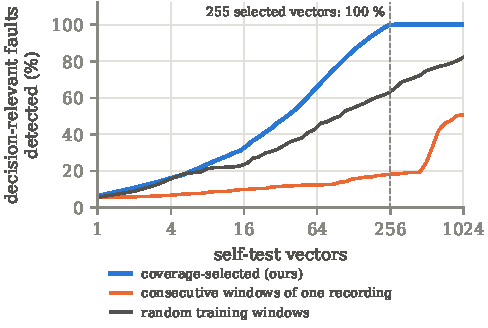
\includegraphics[width=0.72\textwidth]{figures/fault_coverage.pdf}
\caption{Decision-relevant faults detected by the first $m$ self-test vectors}\label{fig:faultcov}
\end{figure}

The natural choice of a test, 1,024 consecutive recorded windows, detects only 50.7\,\% of the faults that change a
decision; the 255 selected windows detect all of them.

\section{Board Test Campaign}\label{sec:res-board}

\begin{table}[H]
\centering\small
\caption{Board test campaign on the KV260 (kit v6 bitstream, Vivado 2026.1)}\label{tab:board}
\begin{tabularx}{\textwidth}{|P{33mm}|L|P{17mm}|}
\hline
\multicolumn{1}{|c|}{\textbf{Step}} & \multicolumn{1}{c|}{\textbf{Measured on the board}} & \multicolumn{1}{c|}{\textbf{Result}}\\
\hline
1 Identity & core version 3, 38 features, 50 LUTs; bitstream loads in 4.4\,s & PASS\\
\hline
2 Self-test & 1,024 of 1,024 vectors correct in 1,028 cycles & PASS\\
\hline
3 Latency & 3 clock cycles (30\,ns) & PASS\\
\hline
4 Replay & all 431,960 windows of 10 recordings through the registers: 0 mismatches at both operating points;
3.2\,\textmu s per window & PASS\\
\hline
5 Detection (10 recordings) & frozen point: 1 of 19 seizures, 0 false alarms in 120\,h; programmable point: 3 of 19,
25 false alarms (equal to simulation) & reported\\
\hline
6 Power & 3.069\,W idle, 3.074\,W with the classifier fed one window per clock (difference within the sensor's
noise) & reported\\
\hline
7 Front end on the Arm & 3 raw recordings: 0 feature and 0 output mismatches, 3,390--4,080 times faster than real
time & PASS\\
\hline
8 Fault injection & all 3,592 faults injected: 0 hardware/software mismatches; all 2,890 decision-relevant faults
detected; 88\,s & PASS\\
\hline
9 Whole detector in the fabric & 9,214 windows from raw samples: 0 feature and 0 output mismatches; engine busy for
exactly the simulated cycles (787,615 / 787,521 / 946,168 per second); 102--124 times faster than real time & PASS\\
\hline
\end{tabularx}
\end{table}

Step 5 covers only the 10 exported recordings of three test patients, as a check that the board reproduces the
software. The first board run found one software bug: the driver wrote ``soft reset'' and ``clear counters'' in the
same register write, and the hardware gives the reset priority, so the counters were not cleared. The driver now writes
them separately (no rebuild was needed).

\section{Analog Front-End Specification}\label{sec:res-afe}

\textbf{One impairment at a time.} Of the 40 families, 29 have a limit, 10 are tolerated even at the most severe level
tested, and one is not tolerated at any level: the ECG low-pass filter fails even at 100\,Hz. Figure~\ref{fig:toleeg}
shows the EEG curves. The detector is most sensitive to mains interference on the EEG (1\,\textmu V of 50\,Hz is
tolerated, 10\,\textmu V is not), so common-mode rejection or a notch matters more than the noise floor.

\begin{figure}[H]
\centering
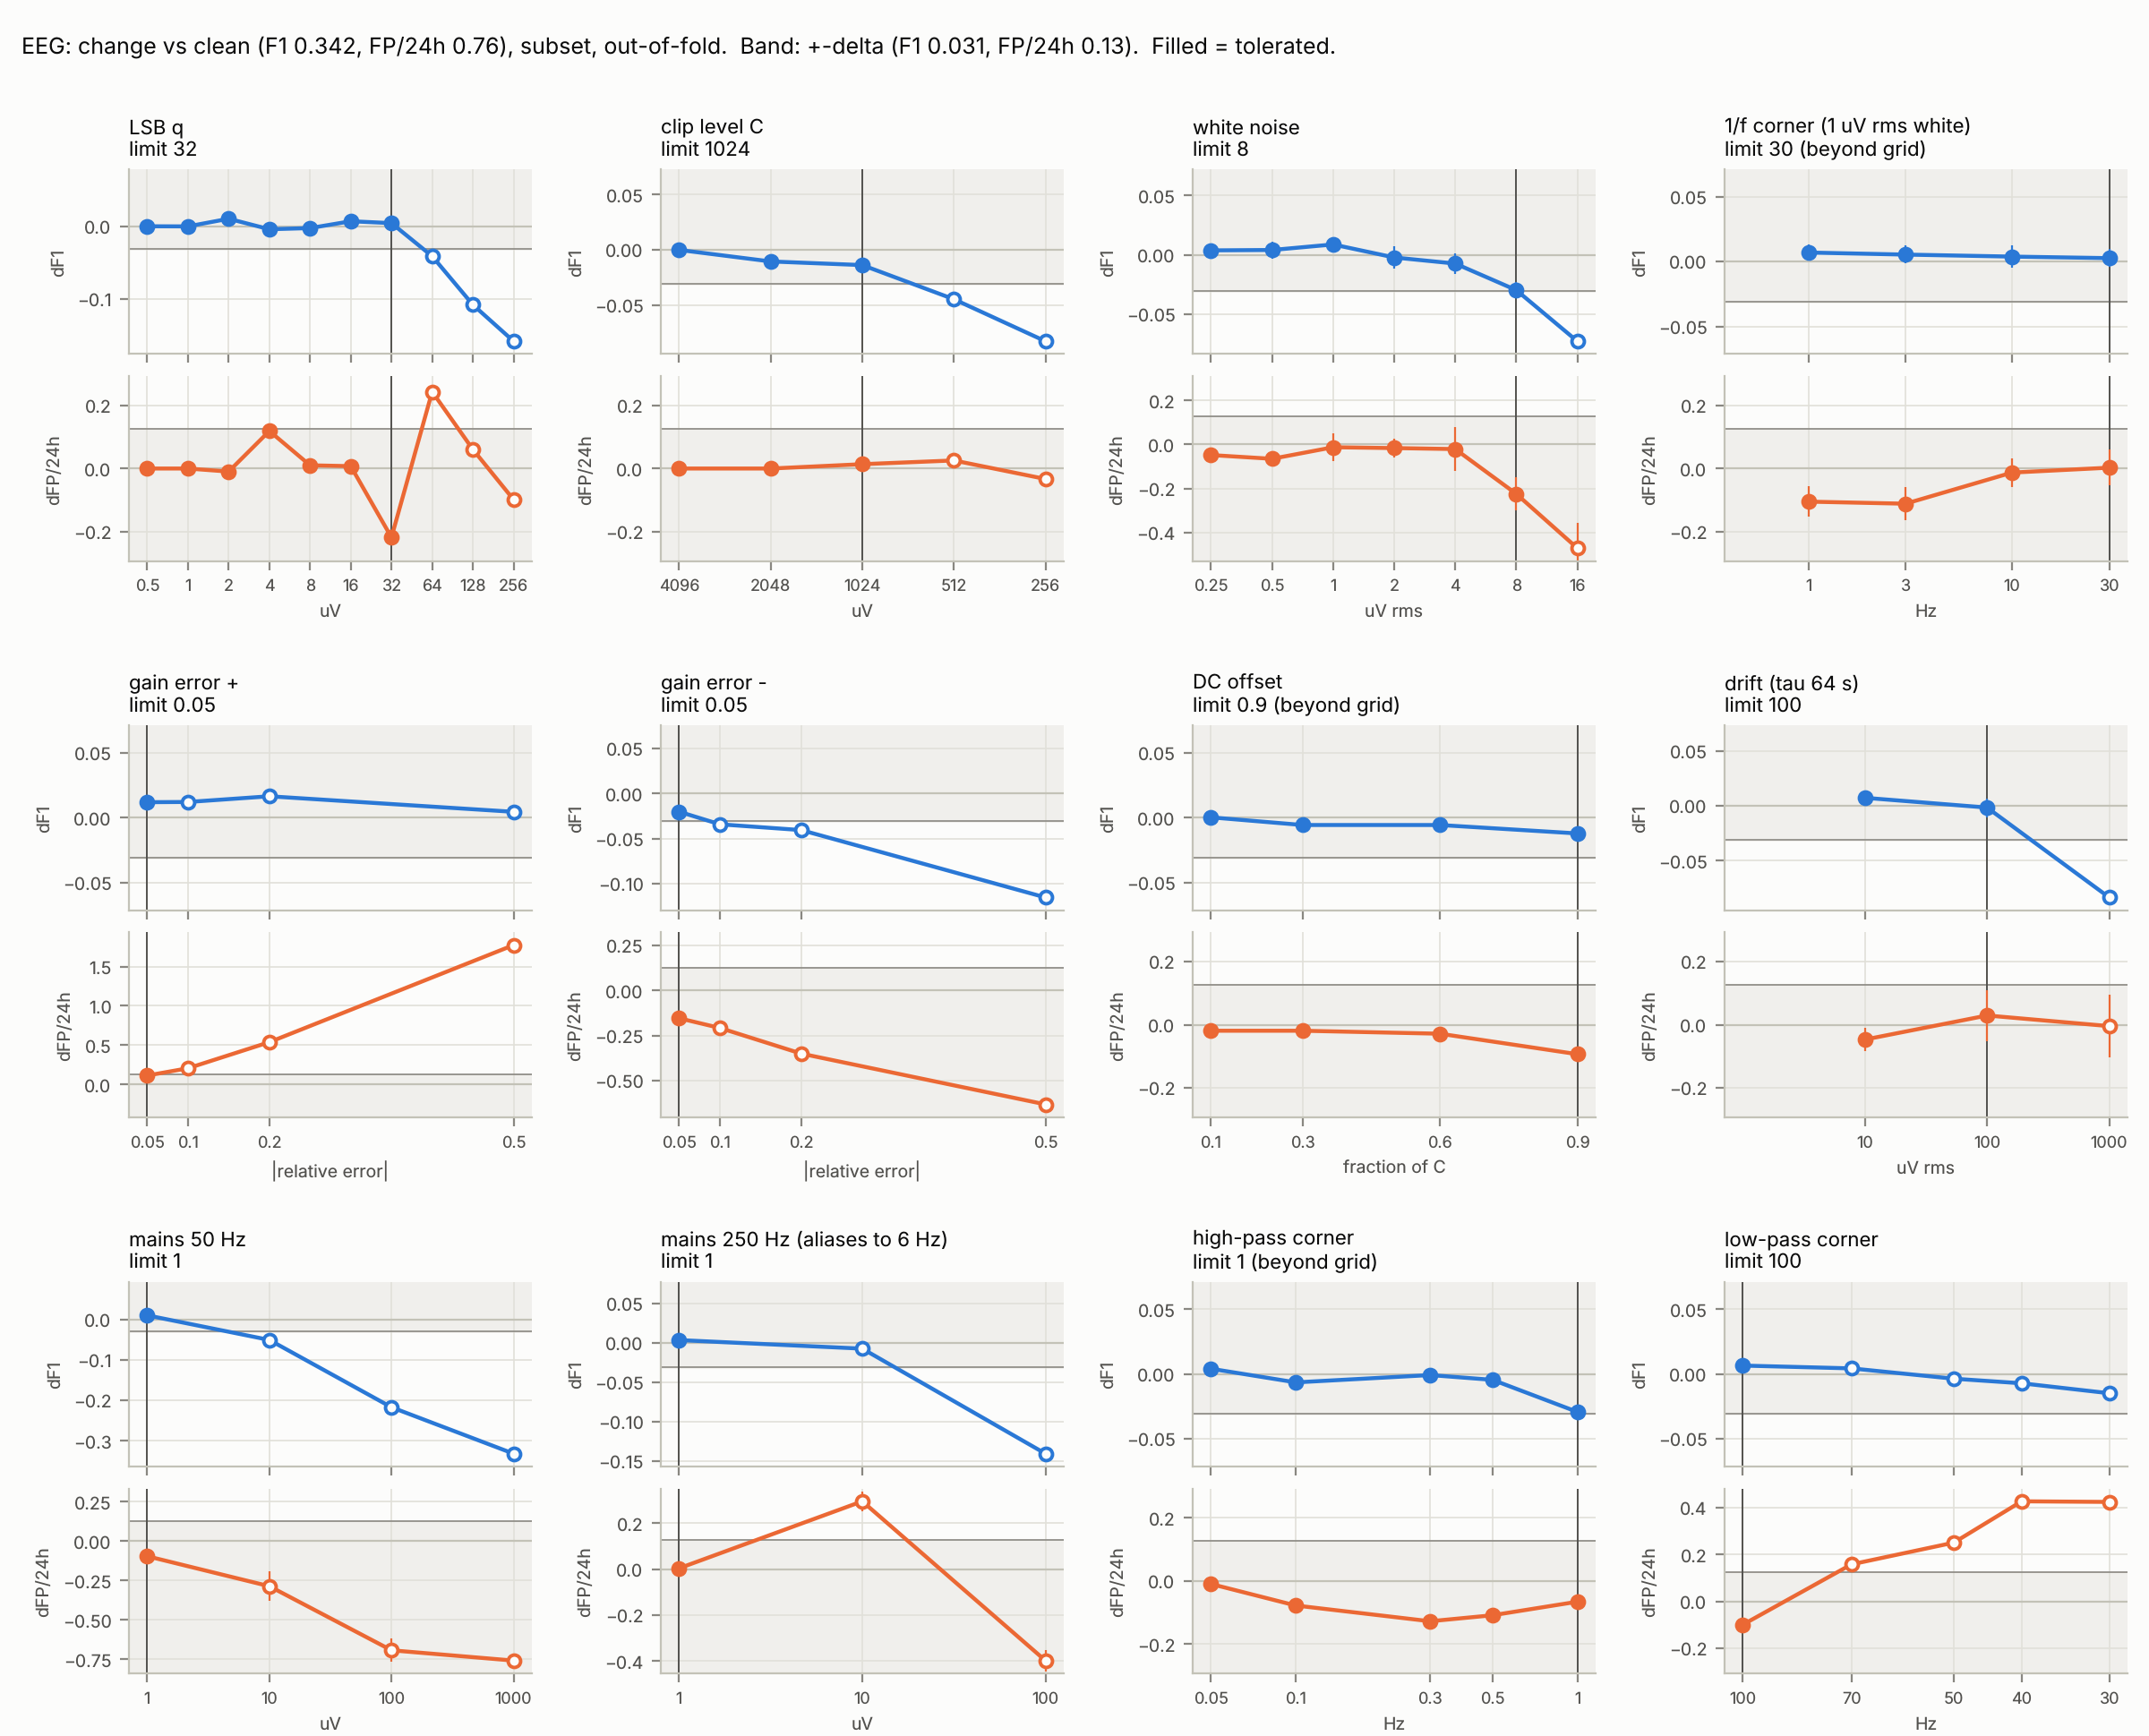
\includegraphics[width=0.95\textwidth]{figures/tolerance_eeg.png}
\caption{EEG tolerance curves on the training subset: change in event-F1 (blue) and false alarms per day (orange)
against each impairment level; filled points are tolerated}\label{fig:toleeg}
\end{figure}

\textbf{All at once.} With every family at its single-impairment limit, the F1 drop was 2.3--2.8 times the allowed
value, because each limit had used the whole error budget by itself. After 22 back-off steps the combined point passed
on the subset, and then on all 8,714.7 training hours with no further step (F1 change $-0.0022$ and $-0.0076$ for the
two signs of gain error; false alarms $+0.105$ and $+0.094$ per day; Wilcoxon $p = 0.48$ and $0.50$).

\begin{table}[H]
\centering\small
\caption{Front-end specification: limit with one impairment at a time and the combined point (all training hours)}\label{tab:afe}
\begin{tabularx}{\textwidth}{|P{20mm}|L|P{36mm}|P{36mm}|}
\hline
\multicolumn{1}{|c|}{\textbf{Signal}} & \multicolumn{1}{c|}{\textbf{Parameter}} & \multicolumn{1}{c|}{\textbf{One at a time}} & \multicolumn{1}{c|}{\textbf{Specification}}\\
\hline
EEG & input noise (0.5--100 Hz) & 4 \textmu V rms & \textbf{1 \textmu V rms}\\
\hline
EEG & ADC step / clip level & 32 \textmu V / 2048 \textmu V & \textbf{4 \textmu V / 2048 \textmu V (10 bits)}\\
\hline
EEG & 50 Hz interference & 1 \textmu V & 1 \textmu V\\
\hline
EEG & high-pass / low-pass corner & 0.5 Hz / 100 Hz & 0.1 Hz / 100 Hz\\
\hline
ECG & input noise & 8 \textmu V rms & \textbf{4 \textmu V rms}\\
\hline
ECG & ADC step / clip level & 32 \textmu V / 1024 \textmu V & \textbf{16 \textmu V / 1024 \textmu V (7 bits)}\\
\hline
ECG & low-pass corner & none tolerated & not included\\
\hline
EMG & input noise & 2 \textmu V rms & \textbf{2 \textmu V rms}\\
\hline
EMG & ADC step / clip level & $\ge$ 256 \textmu V / 1024 \textmu V & \textbf{16 \textmu V / 1024 \textmu V (7 bits)}\\
\hline
Motion & ADC step / noise & 16 LSB / 2 LSB rms & 8 LSB / 1 LSB rms\\
\hline
\end{tabularx}
\end{table}

\begin{table}[H]
\centering\small
\caption{Power of the analog front end at the specification (noise-set amplifier bound for an assumed NEF of 2, 3 and 5; ADC
power from the Murmann survey)}\label{tab:afepower}
\begin{tabular}{|l|c|c|c|c|c|}
\hline
\multicolumn{1}{|c|}{\textbf{Channels}} & \textbf{Noise density} & \textbf{NEF 2} & \textbf{NEF 3} & \textbf{NEF 5} & \textbf{ADC bits}\\
\hline
EEG (2), per channel & 100 nV/$\sqrt{\mathrm{Hz}}$ & 482 nW & 1.08 \textmu W & 3.01 \textmu W & 10\\
\hline
ECG (1) & 401 nV/$\sqrt{\mathrm{Hz}}$ & 30.1 nW & 67.8 nW & 188 nW & 7\\
\hline
EMG (1) & 201 nV/$\sqrt{\mathrm{Hz}}$ & 120 nW & 271 nW & 753 nW & 7\\
\hline
\textbf{All 4 channels} & & \textbf{1.11 \textmu W} & \textbf{2.51 \textmu W} & \textbf{6.97 \textmu W} & \\
\hline
\end{tabular}
\end{table}

The ADCs of the lowest-power real low-rate designs in the survey add about 941\,nW for all channels. The analog front end
therefore needs a few microwatts, set mainly by the EEG amplifiers: tightening the EEG noise from 4 to 1\,\textmu V rms
costs 16 times the amplifier current at the same NEF.

\textbf{FPGA impairment emulator.} The Verilog emulator matched the Python impairment model word for word in 11 test
cases of 70,000 samples each (0 mismatches; flipping one seed bit changed 65,702 of 70,000 words, which shows the
comparison works), both on its own and behind AXI4-Lite. It takes 4,713 LUTs (5,117 with AXI) in Yosys. Its run on the
board is still to be done.

\section{Live Demonstration and Doctor Alert}\label{sec:res-demo}

On the board, recorded test-patient signals stream second by second through the fabric; the alarm fires during the
seizure and the red LED and the buzzer turn on. Figure~\ref{fig:dashboard} shows the dashboard and
Figure~\ref{fig:alertpage} the doctor's page.

\begin{figure}[H]
\centering
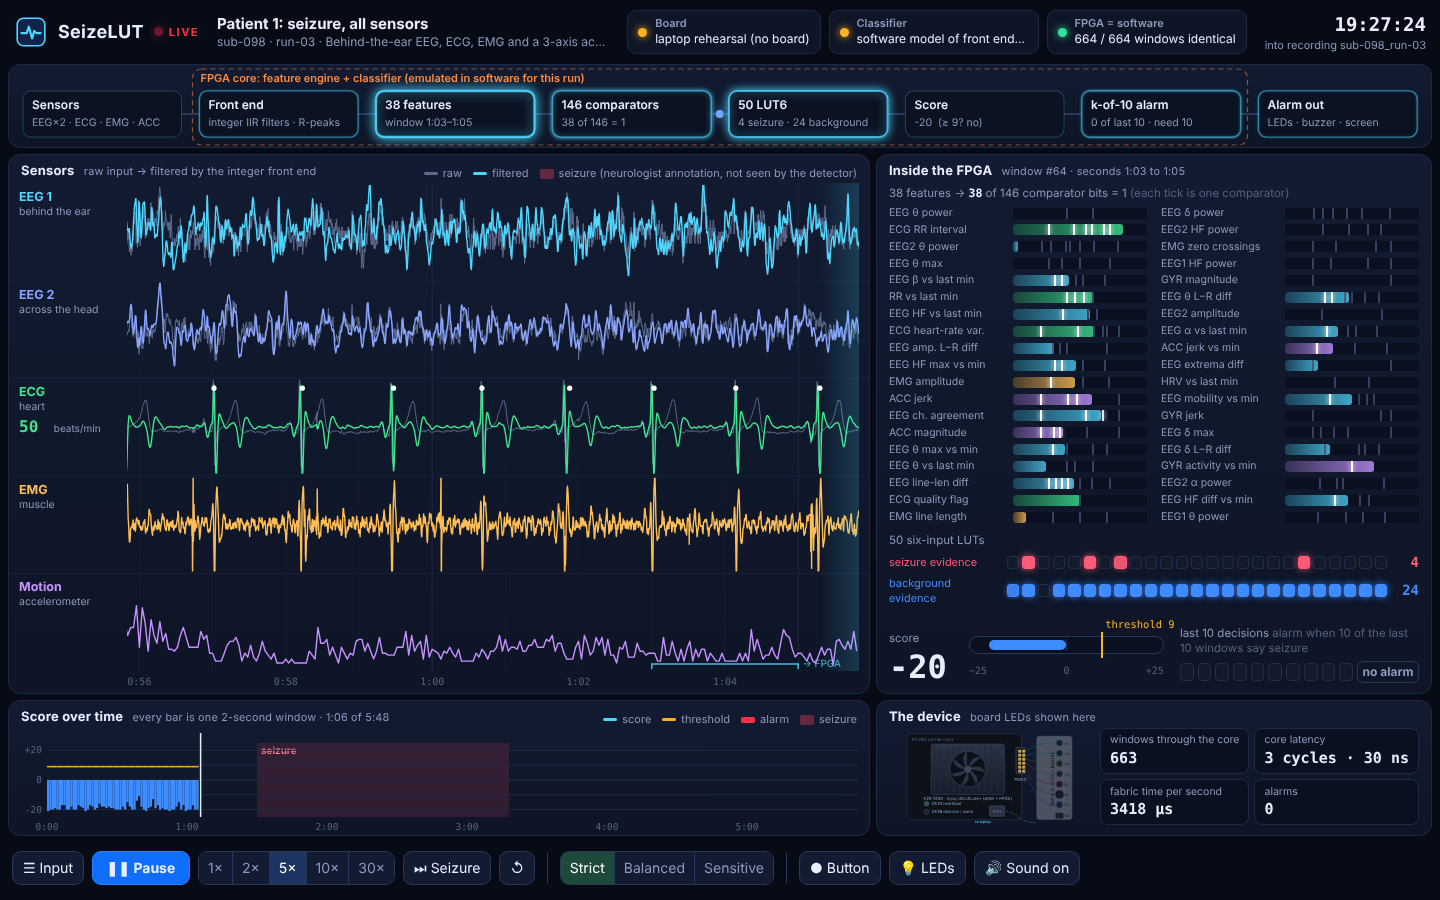
\includegraphics[width=\textwidth]{figures/dashboard_rehearsal.png}
\caption{Live dashboard: signals, features, comparator bits, LUT votes, score and alarm, with the check that the FPGA
equals the software (laptop rehearsal with the software model of the core; on the board the same page shows the
FPGA)}\label{fig:dashboard}
\end{figure}

\begin{figure}[H]
\centering
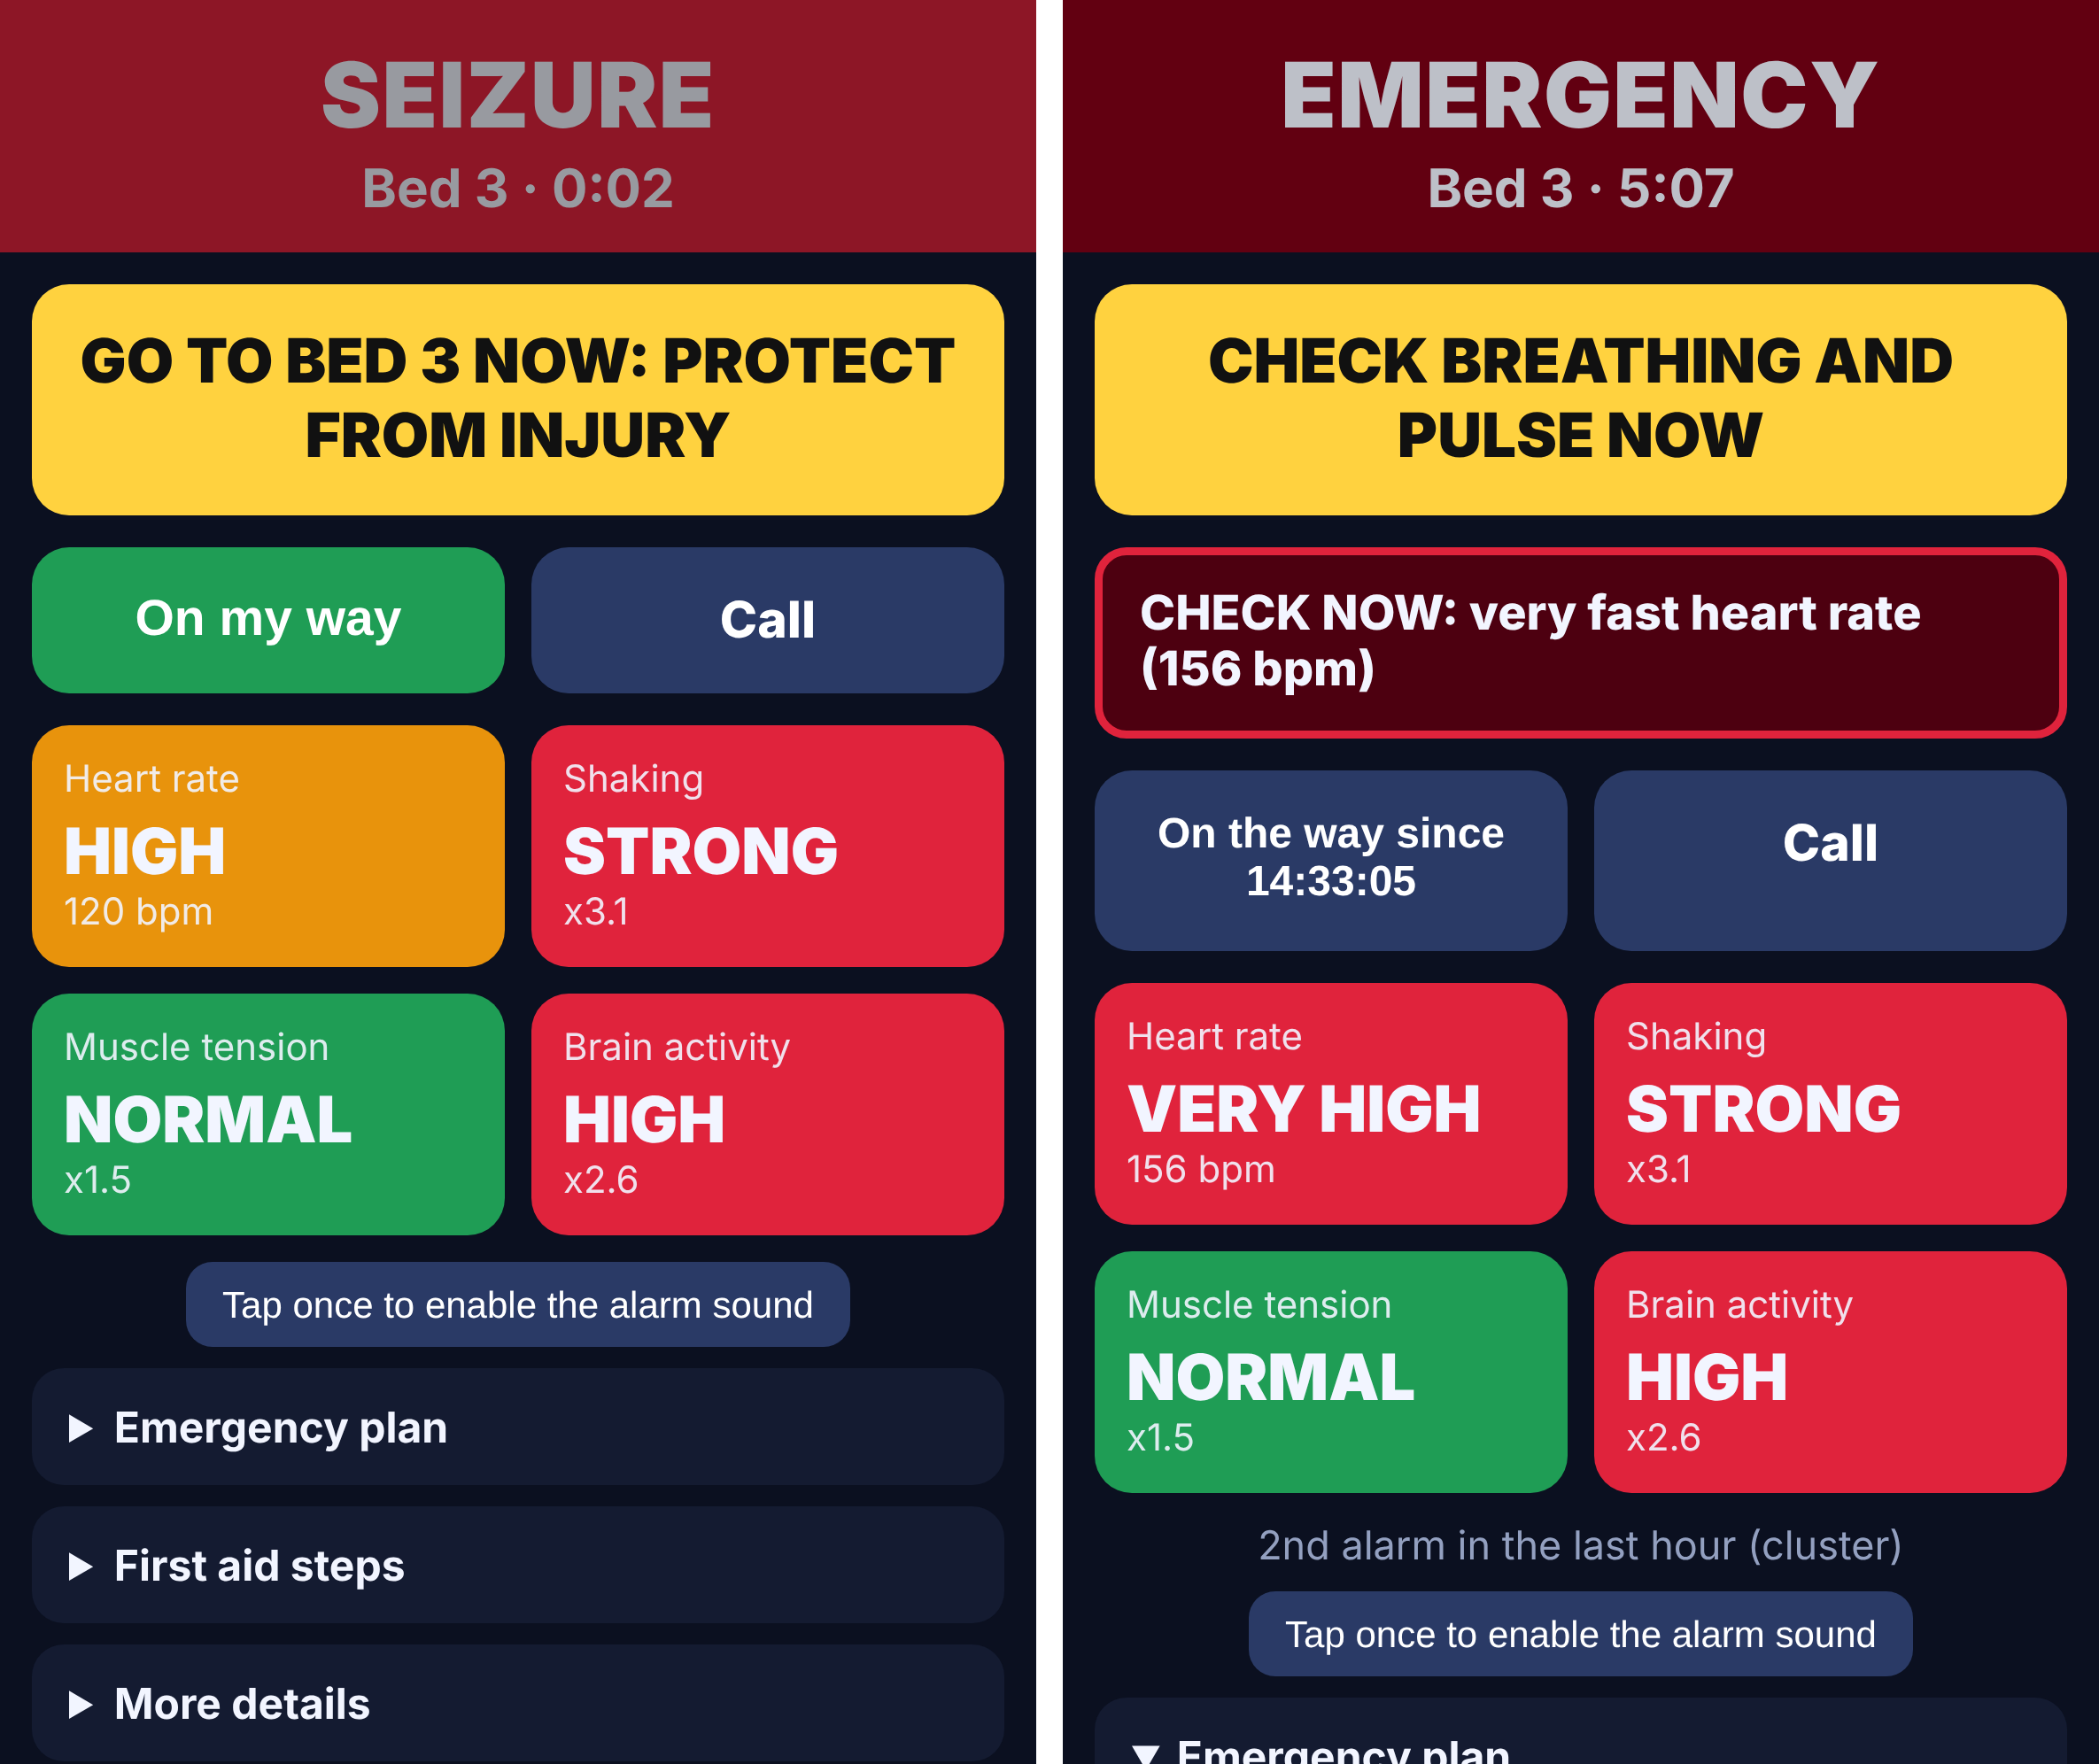
\includegraphics[width=0.85\textwidth]{figures/alert_page.png}
\caption{The doctor's page at a new seizure (left) and in an emergency after 5 minutes (right)}\label{fig:alertpage}
\end{figure}

The alert was tested on the emulated board through a virtual serial port: alarm start, updates, end after 30\,s of
quiet, escalation at 2, 5, 6 and 7 minutes (none after the alarm stops), clusters, and the acknowledgement coming back.
The ESP32 program passes a syntax check and the page was rendered at iPhone size. The test on the ESP32 itself, with a
real iPhone, is the next step.
